\begin{frame}{What a Vision-Language Model Does}
  \begin{itemize}\footnotesize\itemsep0.3em
    \item A \textbf{vision-language model (VLM)} takes one or more images together with text and returns either a \textbf{match score or embedding}, as CLIP does, or \textbf{new text}, as the LLaVA-style assistant built on a large language model (LLM) does. CLIP was covered earlier; the LLaVA-style assistant is built up in this lecture.
  \end{itemize}

  {\centering
  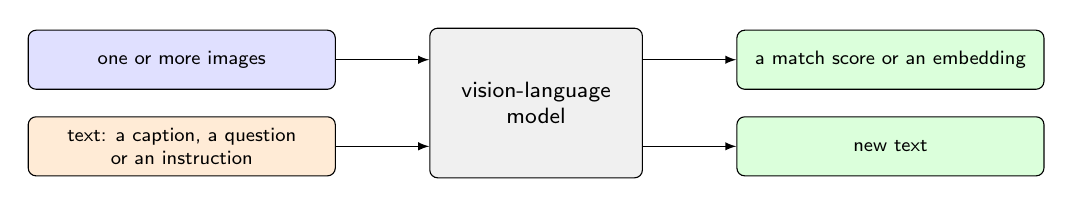
\begin{tikzpicture}[font=\sffamily\scriptsize, >=latex,
      box/.style={draw, rounded corners=0.1cm, align=center, minimum height=0.75cm}]
    \node[box, fill=blue!12, minimum width=3.9cm] (img) at (0,0.55) {one or more images};
    \node[box, fill=orange!16, minimum width=3.9cm] (txt) at (0,-0.55) {text: a caption, a question\\or an instruction};
    \node[box, fill=gray!12, font=\sffamily\footnotesize, minimum width=2.7cm, minimum height=1.9cm] (vlm) at (4.5,0) {vision-language\\model};
    \node[box, fill=green!14, minimum width=3.9cm] (score) at (9.0,0.55) {a match score or an embedding};
    \node[box, fill=green!14, minimum width=3.9cm] (gen) at (9.0,-0.55) {new text};
    \draw[->] (img.east) -- (img.east -| vlm.west);
    \draw[->] (txt.east) -- (txt.east -| vlm.west);
    \draw[->] (vlm.east |- score.west) -- (score.west);
    \draw[->] (vlm.east |- gen.west) -- (gen.west);
  \end{tikzpicture}\par}
  \vspace{0.3em}
  \begin{columns}[T,onlytextwidth]
    \column{0.40\textwidth}
      {\scriptsize\textbf{Output: a score or an embedding}\par}
      \begin{itemize}\scriptsize\itemsep0.15em
        \item \textbf{Retrieval:} find the caption for an image, or the image for a caption.
        \item \textbf{Zero-shot classification:} rank class-name prompts by match score.
      \end{itemize}
    \column{0.58\textwidth}
      {\scriptsize\textbf{Output: text}\par}
      \begin{itemize}\scriptsize\itemsep0.15em
        \item \textbf{Captioning:} describe the image in a sentence.
        \item \textbf{Visual question answering (VQA):} answer questions.
        \item \textbf{Document understanding:} read text, tables and charts.
        \item \textbf{Grounding:} give a region's box as text, e.g.\ $(x_1,y_1),(x_2,y_2)$.
        \item \textbf{Visual chat:} follow multi-turn instructions about images.
      \end{itemize}
  \end{columns}
  \vspace{0.2em}
  {\scriptsize Box format (corners scaled to $[0,1000)$): Bai et al., ``Qwen-VL: A Versatile Vision-Language Model for Understanding, Localization, Text Reading, and Beyond,'' 2023, \href{https://arxiv.org/abs/2308.12966v3}{arXiv:2308.12966v3}, Sec.~2.2.\par}
\end{frame}

\begin{frame}{Vision-Language Tasks and Their Metrics}

  {\centering\scriptsize\setlength{\tabcolsep}{4pt}
  \begin{tabular}{>{\raggedright\arraybackslash}p{1.9cm} >{\raggedright\arraybackslash}p{3.0cm} >{\raggedright\arraybackslash}p{1.6cm} >{\raggedright\arraybackslash}p{5.9cm}}
    \toprule
    \textbf{Task} & \textbf{Benchmark} & \textbf{Metric} & \textbf{How one prediction is scored} \\
    \midrule
    Retrieval & Flickr30K (1K test), COCO (5K test) & Recall@$K$ & 1 if a paired caption (image query) or the paired image (caption query) is in the top $K$ \\
    \addlinespace[0.2em]
    Zero-shot classification & ImageNet & top-1 accuracy & 1 if the best-matching class prompt names the true class \\
    \addlinespace[0.2em]
    Captioning & COCO (5K test) & CIDEr & consensus with the 5 human captions \\
    \addlinespace[0.2em]
    VQA & VQAv2 & VQA accuracy & $\min(n/3,\,1)$ for $n$ matching annotators, averaged over the 10 subsets of 9 annotators \\
    \addlinespace[0.2em]
    Document VQA & DocVQA (50K questions, 12,767 images) & ANLS & best $s = 1-\mathrm{NL}(a_j, o)$ over the reference answers $a_j$, with $s = 0$ when $\mathrm{NL} \geq 0.5$ \\
    \bottomrule
  \end{tabular}\par}
  \vspace{0.3em}
  {\scriptsize Recall@$K$, top-1 accuracy and CIDEr were covered earlier; Flickr30K has 31K images with 5 captions each. \textbf{VQA accuracy:} after averaging, an answer given by 1, 2, 3 or $\geq 4$ of the 10 annotators scores 0.3, 0.6, 0.9 or 1. \textbf{ANLS} (average normalized Levenshtein similarity) averages the best $s$ over all questions; $o$ is the model's answer and NL the edit distance (fewest character insertions, deletions and substitutions) scaled to $[0,1]$, so a few misread characters keep most of the credit.\par}
  \vspace{0.3em}
  {\scriptsize Karpathy and Fei-Fei, ``Deep Visual-Semantic Alignments for Generating Image Descriptions,'' CVPR 2015, \href{https://openaccess.thecvf.com/content_cvpr_2015/papers/Karpathy_Deep_Visual-Semantic_Alignments_2015_CVPR_paper.pdf}{OpenAccess}, Sec.~4. Antol et al., ``VQA: Visual Question Answering,'' ICCV 2015, \href{https://openaccess.thecvf.com/content_iccv_2015/papers/Antol_VQA_Visual_Question_ICCV_2015_paper.pdf}{OpenAccess}, Sec.~3 and footnote~2; scores from the official code, \href{https://visualqa.org/evaluation.html}{visualqa.org/evaluation.html}. Biten et al., ``Scene Text Visual Question Answering,'' ICCV 2019, \href{https://arxiv.org/abs/1905.13648v2}{arXiv:1905.13648v2}, Sec.~3.4. Mathew et al., ``DocVQA: A Dataset for VQA on Document Images,'' WACV 2021, \href{https://arxiv.org/abs/2007.00398v3}{arXiv:2007.00398v3}, Secs.~1 and~5.1.\par}
\end{frame}

\begin{frame}{Three Ways to Combine Vision and Language}

  {\centering
  \resizebox{\textwidth}{!}{%
  \begin{tikzpicture}[font=\sffamily\scriptsize, >=latex,
      box/.style={draw, rounded corners=0.1cm, align=center, minimum height=0.45cm, inner sep=2pt},
      vis/.style={box, fill=blue!12},
      lang/.style={box, fill=orange!16},
      res/.style={box, fill=white},
      lbl/.style={inner sep=1pt},
      note/.style={anchor=north, text width=4.3cm, align=flush left, inner sep=0pt}]
    \draw[rounded corners=0.15cm, draw=teal!70!black, fill=teal!6] (0,0) rectangle (4.5,3.45);
    \node[font=\sffamily\scriptsize\bfseries, text=teal!60!black] at (2.25,3.2) {(a) Dual encoder};
    \node at (2.25,2.85) {CLIP, ALIGN, SigLIP};
    \node[lbl] (ai) at (1.1,0.2) {image};
    \node[lbl] (at) at (3.4,0.2) {text};
    \node[vis, minimum width=1.5cm, minimum height=0.9cm] (aie) at (1.1,1.0) {image\\encoder};
    \node[lang, minimum width=1.5cm, minimum height=0.9cm] (ate) at (3.4,1.0) {text\\encoder};
    \node[res] (ao) at (2.25,2.3) {match score $\mathbf{v}^{\top}\mathbf{t}$};
    \draw[->] (ai) -- (aie);
    \draw[->] (at) -- (ate);
    \draw[->] (aie.north) -- node[left] {$\mathbf{v}$} ($(ao.south)+(-0.55,0)$);
    \draw[->] (ate.north) -- node[right] {$\mathbf{t}$} ($(ao.south)+(0.55,0)$);
    \node[note] at (2.25,-0.15) {Image embeddings are computed once and indexed, so a text query costs one encoder pass plus dot products. Image and text meet only in that product; no text output.};
    \begin{scope}[xshift=4.75cm]
      \draw[rounded corners=0.15cm, draw=violet!70!black, fill=violet!5] (0,0) rectangle (4.5,3.45);
      \node[font=\sffamily\scriptsize\bfseries, text=violet!70!black] at (2.25,3.2) {(b) Fusion model};
      \node at (2.25,2.85) {ALBEF, BLIP, CoCa};
      \node[lbl] (bi) at (0.9,0.2) {image};
      \node[lbl] (bt) at (3.3,0.2) {text};
      \node[vis, minimum width=1.3cm, minimum height=0.9cm] (bie) at (0.9,1.0) {image\\encoder};
      \node[lang, text width=2.1cm, minimum height=1.15cm] (bf) at (3.3,1.12) {text layers with\\cross-attention};
      \node[res] (bo) at (3.3,2.3) {score or caption};
      \draw[->] (bi) -- (bie);
      \draw[->] (bt) -- (bf);
      \draw[->] (bie.east) -- (bie.east -| bf.west);
      \draw[->] (bf) -- (bo);
      \node[note] at (2.25,-0.15) {Text layers cross-attend to image features; BLIP and CoCa also write captions. One joint pass per pair, so ALBEF re-ranks only the top $k$ found by dot products.};
    \end{scope}
    \begin{scope}[xshift=9.5cm]
      \draw[rounded corners=0.15cm, draw=green!50!black, fill=green!5] (0,0) rectangle (4.5,3.45);
      \node[font=\sffamily\scriptsize\bfseries, text=green!40!black] at (2.25,3.2) {(c) LLM-based};
      \node at (2.25,2.85) {Flamingo, BLIP-2, LLaVA, Qwen-VL};
      \node[lbl] (ci) at (0.85,0.2) {image};
      \node[lbl] (ct) at (3.3,0.2) {text};
      \node[vis, minimum width=1.3cm, minimum height=0.7cm] (cv) at (0.85,0.85) {vision\\encoder};
      \node[vis, minimum width=1.3cm] (cc) at (0.85,1.65) {connector};
      \node[box, fill=gray!15, minimum width=1.6cm, minimum height=1.35cm] (cl) at (3.3,1.2) {LLM};
      \node[res] (co) at (3.3,2.3) {generated text};
      \draw[->] (ci) -- (cv);
      \draw[->] (cv) -- (cc);
      \draw[->] (cc.east) -- node[below, align=center] {visual\\tokens} (cc.east -| cl.west);
      \draw[->] (ct) -- (cl);
      \draw[->] (cl) -- (co);
      \node[note] at (2.25,-0.15) {Open-ended text with the LLM's knowledge and instruction following. Images enter as extra input tokens or via added cross-attention layers (Flamingo); each adds LLM compute.};
    \end{scope}
  \end{tikzpicture}}\par}
  \vspace{0.3em}
  {\scriptsize Left to right, image and text interact more deeply and each image-text pair costs more to process.\par}
  \vspace{0.2em}
  {\scriptsize Top-$k$ re-ranking: Li et al., ``Align before Fuse: Vision and Language Representation Learning with Momentum Distillation,'' NeurIPS 2021, \href{https://arxiv.org/abs/2107.07651v2}{arXiv:2107.07651v2}, Sec.~5.\par}
\end{frame}

\begin{frame}{The Language Side: Decoder-Only LLMs}

  {\centering
  \resizebox{\textwidth}{!}{%
  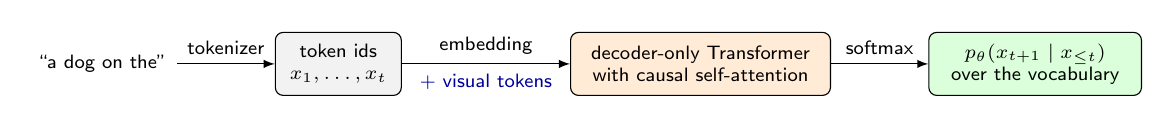
\begin{tikzpicture}[font=\sffamily\scriptsize, >=latex,
      box/.style={draw, rounded corners=0.1cm, align=center, minimum height=0.8cm, inner sep=2pt}]
    \node (t0) at (0.75,0) {``a dog on the''};
    \node[box, fill=gray!10, minimum width=1.6cm] (ids) at (3.75,0) {token ids\\$x_1,\ldots,x_t$};
    \node[box, fill=orange!16, minimum width=3.3cm] (dec) at (8.35,0) {decoder-only Transformer\\with causal self-attention};
    \node[box, fill=green!14, minimum width=2.7cm] (out) at (12.6,0) {$p_\theta(x_{t+1}\mid x_{\leq t})$\\over the vocabulary};
    \draw[->] (t0) -- node[above] {tokenizer} (ids);
    \draw[->] (ids) -- node[above] {embedding} node[below, text=blue!60!black] {+ visual tokens} (dec);
    \draw[->] (dec) -- node[above] {softmax} (out);
  \end{tikzpicture}}\par}
  \vspace{0.2em}
  \begin{itemize}\footnotesize\itemsep0.3em
    \item \textbf{Tokenizer:} cuts text into subword tokens from a fixed vocabulary (Qwen2: 151,643 regular tokens); an embedding table maps each token id to a vector. LLaVA-style models add visual tokens here.
    \item \textbf{Pretraining:} next-token prediction on large text corpora, the autoregressive likelihood (covered earlier); the causal mask lets position $t$ see only $x_{\leq t}$:
    \[ \mathcal{L}(\theta) = -\textstyle\sum_{t=1}^{T} \log p_\theta(x_t \mid x_{<t}) \]
    $x_t$: the $t$-th token; $x_{<t}$: the tokens before it; $T$: sequence length; $\theta$: the model's weights.
    \item \textbf{Instruction tuning:} ``finetuning language models on a collection of datasets described via instructions'' (FLAN), which ``substantially improves zero-shot performance on unseen tasks''. Chat models such as Vicuna compute the loss on the response tokens only; the instruction serves as context.
  \end{itemize}
  \vspace{0.1em}
  {\scriptsize Wei et al., ``Finetuned Language Models Are Zero-Shot Learners,'' ICLR 2022, \href{https://arxiv.org/abs/2109.01652v5}{arXiv:2109.01652v5}, Abstract. The Vicuna Team, ``Vicuna: An Open-Source Chatbot Impressing GPT-4 with 90\%* ChatGPT Quality,'' LMSYS blog, 30 Mar.\ 2023, \href{https://www.lmsys.org/blog/2023-03-30-vicuna/}{lmsys.org/blog/2023-03-30-vicuna}. Yang et al., ``Qwen2 Technical Report,'' 2024, \href{https://arxiv.org/abs/2407.10671v4}{arXiv:2407.10671v4}, Sec.~2.1.\par}
\end{frame}

\begin{frame}{The LLMs Inside This Lecture's VLMs}

  {\centering\scriptsize\setlength{\tabcolsep}{3pt}
  \begin{tabular}{>{\raggedright\arraybackslash}p{2.1cm} >{\raggedright\arraybackslash}p{1.6cm} >{\raggedright\arraybackslash}p{4.2cm} >{\raggedright\arraybackslash}p{1.9cm} >{\raggedright\arraybackslash}p{2.6cm}}
    \toprule
    \textbf{LLM} & \textbf{From} & \textbf{What it is} & \textbf{Used by} & \textbf{Source} \\
    \midrule
    Chinchilla 1.4B, 7B, 70B & DeepMind, 2022 & decoder-only; the 70B model was trained on 1.4T tokens & Flamingo (frozen) & Hoffmann et al., \href{https://arxiv.org/abs/2203.15556v1}{arXiv:2203.15556v1} \\
    \addlinespace[0.15em]
    OPT 2.7B, 6.7B & Meta AI, 2022 & decoder-only; open suite from 125M to 175B & BLIP-2 (frozen) & Zhang et al., \href{https://arxiv.org/abs/2205.01068v4}{arXiv:2205.01068v4} \\
    \addlinespace[0.15em]
    FlanT5 XL, XXL (3B, 11B) & Google, 2022 & encoder-decoder T5, instruction-tuned on 1,836 tasks & BLIP-2 (frozen) & Chung et al., \href{https://arxiv.org/abs/2210.11416v5}{arXiv:2210.11416v5} \\
    \addlinespace[0.15em]
    Vicuna 7B, 13B & LMSYS, Mar.\ 2023 & LLaMA (Meta AI) fine-tuned on about 70K ChatGPT conversations shared by users & LLaVA & LMSYS blog; Touvron et al., \href{https://arxiv.org/abs/2302.13971v1}{arXiv:2302.13971v1} \\
    \addlinespace[0.15em]
    Qwen2 & Alibaba, 2024 & decoder-only; open weights, 0.5B to 72B & Qwen2-VL & Yang et al., \href{https://arxiv.org/abs/2407.10671v4}{arXiv:2407.10671v4} \\
    \addlinespace[0.15em]
    Qwen2.5 & Alibaba, 2024 & decoder-only; 0.5B to 72B, 18T pretraining tokens & Qwen2.5-VL & Qwen Team, \href{https://arxiv.org/abs/2412.15115v2}{arXiv:2412.15115v2} \\
    \bottomrule
  \end{tabular}\par}
  \vspace{0.4em}
  {\footnotesize \textbf{Frozen:} the LLM's weights are not updated when the VLM is trained; given no image, Flamingo falls back to plain language-model behavior.\par}
  \vspace{0.3em}
  {\scriptsize Which LLM each VLM uses: Alayrac et al., \href{https://arxiv.org/abs/2204.14198v2}{arXiv:2204.14198v2}, Sec.~2.2 and App.~D.2.2; Li et al., \href{https://arxiv.org/abs/2301.12597v3}{arXiv:2301.12597v3}, Sec.~3.4; Liu et al., \href{https://arxiv.org/abs/2304.08485v2}{arXiv:2304.08485v2}, Sec.~4.1; Wang et al., \href{https://arxiv.org/abs/2409.12191v2}{arXiv:2409.12191v2}, Sec.~2.1; Bai et al., \href{https://arxiv.org/abs/2502.13923v1}{arXiv:2502.13923v1}, Sec.~2.1.\par}
\end{frame}

\begin{frame}{A Short History, 2021--2025}

  {\centering
  \resizebox{\textwidth}{!}{%
  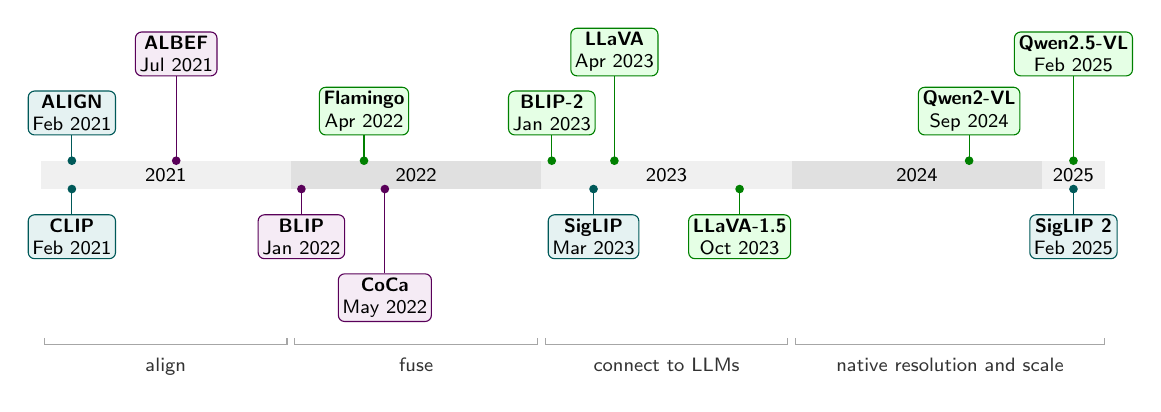
\begin{tikzpicture}[font=\sffamily\scriptsize, >=latex,
      evt/.style={draw, rounded corners=0.08cm, align=center, inner sep=1.5pt},
      dual/.style={evt, draw=teal!70!black, fill=teal!10},
      fuse/.style={evt, draw=violet!70!black, fill=violet!8},
      llm/.style={evt, draw=green!50!black, fill=green!10}]
    % x = 0.3 + 0.265 (m + 0.5), m = months since January 2021: each dot sits mid-month of the
    % arXiv v1 date. Labels alternate above/below at two heights (|y| = 0.5 or 1.25) so none overlap.
    \fill[gray!12] (0.3,-0.18) rectangle (3.48,0.18);
    \fill[gray!24] (3.48,-0.18) rectangle (6.66,0.18);
    \fill[gray!12] (6.66,-0.18) rectangle (9.84,0.18);
    \fill[gray!24] (9.84,-0.18) rectangle (13.02,0.18);
    \fill[gray!12] (13.02,-0.18) rectangle (13.815,0.18);
    \node at (1.89,0) {2021};
    \node at (5.07,0) {2022};
    \node at (8.25,0) {2023};
    \node at (11.43,0) {2024};
    \node at (13.4175,0) {2025};
    \draw[teal!70!black] (0.6975,0.18) -- (0.6975,0.5);
    \fill[teal!70!black] (0.6975,0.18) circle (0.055);
    \node[dual, anchor=south] at (0.6975,0.5) {\textbf{ALIGN}\\Feb 2021};
    \draw[violet!70!black] (2.0225,0.18) -- (2.0225,1.25);
    \fill[violet!70!black] (2.0225,0.18) circle (0.055);
    \node[fuse, anchor=south] at (2.0225,1.25) {\textbf{ALBEF}\\Jul 2021};
    \draw[green!50!black] (4.4075,0.18) -- (4.4075,0.5);
    \fill[green!50!black] (4.4075,0.18) circle (0.055);
    \node[llm, anchor=south] at (4.4075,0.5) {\textbf{Flamingo}\\Apr 2022};
    \draw[green!50!black] (6.7925,0.18) -- (6.7925,0.5);
    \fill[green!50!black] (6.7925,0.18) circle (0.055);
    \node[llm, anchor=south] at (6.7925,0.5) {\textbf{BLIP-2}\\Jan 2023};
    \draw[green!50!black] (7.5875,0.18) -- (7.5875,1.25);
    \fill[green!50!black] (7.5875,0.18) circle (0.055);
    \node[llm, anchor=south] at (7.5875,1.25) {\textbf{LLaVA}\\Apr 2023};
    \draw[green!50!black] (12.0925,0.18) -- (12.0925,0.5);
    \fill[green!50!black] (12.0925,0.18) circle (0.055);
    \node[llm, anchor=south] at (12.0925,0.5) {\textbf{Qwen2-VL}\\Sep 2024};
    \draw[green!50!black] (13.4175,0.18) -- (13.4175,1.25);
    \fill[green!50!black] (13.4175,0.18) circle (0.055);
    \node[llm, anchor=south] at (13.4175,1.25) {\textbf{Qwen2.5-VL}\\Feb 2025};
    \draw[teal!70!black] (0.6975,-0.18) -- (0.6975,-0.5);
    \fill[teal!70!black] (0.6975,-0.18) circle (0.055);
    \node[dual, anchor=north] at (0.6975,-0.5) {\textbf{CLIP}\\Feb 2021};
    \draw[violet!70!black] (3.6125,-0.18) -- (3.6125,-0.5);
    \fill[violet!70!black] (3.6125,-0.18) circle (0.055);
    \node[fuse, anchor=north] at (3.6125,-0.5) {\textbf{BLIP}\\Jan 2022};
    \draw[violet!70!black] (4.6725,-0.18) -- (4.6725,-1.25);
    \fill[violet!70!black] (4.6725,-0.18) circle (0.055);
    \node[fuse, anchor=north] at (4.6725,-1.25) {\textbf{CoCa}\\May 2022};
    \draw[teal!70!black] (7.3225,-0.18) -- (7.3225,-0.5);
    \fill[teal!70!black] (7.3225,-0.18) circle (0.055);
    \node[dual, anchor=north] at (7.3225,-0.5) {\textbf{SigLIP}\\Mar 2023};
    \draw[green!50!black] (9.1775,-0.18) -- (9.1775,-0.5);
    \fill[green!50!black] (9.1775,-0.18) circle (0.055);
    \node[llm, anchor=north] at (9.1775,-0.5) {\textbf{LLaVA-1.5}\\Oct 2023};
    \draw[teal!70!black] (13.4175,-0.18) -- (13.4175,-0.5);
    \fill[teal!70!black] (13.4175,-0.18) circle (0.055);
    \node[dual, anchor=north] at (13.4175,-0.5) {\textbf{SigLIP 2}\\Feb 2025};
    \draw[gray!70] (0.35,-2.07) -- (0.35,-2.15) -- (3.43,-2.15) -- (3.43,-2.07);
    \draw[gray!70] (3.53,-2.07) -- (3.53,-2.15) -- (6.61,-2.15) -- (6.61,-2.07);
    \draw[gray!70] (6.71,-2.07) -- (6.71,-2.15) -- (9.79,-2.15) -- (9.79,-2.07);
    \draw[gray!70] (9.89,-2.07) -- (9.89,-2.15) -- (13.815,-2.15) -- (13.815,-2.07);
    \node[anchor=north, text=gray!40!black] at (1.89,-2.2) {align};
    \node[anchor=north, text=gray!40!black] at (5.07,-2.2) {fuse};
    \node[anchor=north, text=gray!40!black] at (8.25,-2.2) {connect to LLMs};
    \node[anchor=north, text=gray!40!black] at (11.85,-2.2) {native resolution and scale};
  \end{tikzpicture}}\par}
  \vspace{0.3em}
  {\scriptsize Box color gives the family: \textcolor{teal!70!black}{\textbf{dual encoder}}, \textcolor{violet!70!black}{\textbf{fusion model}}, \textcolor{green!45!black}{\textbf{LLM-based}}. The brackets mark rough eras; the colors show that the families overlap in time. Each box sits at the month of the paper's first arXiv version (v1); full references are at the end.\par}
\end{frame}
